We are given video feed from a front facing monocular camera. We assume that features like car detections, point tracks, lane detections, ground plane and ego-motion are already available. We also use GPS and Map as a given input to the system. With this available information our goal is to find position, orientation and dimensions different participants in the scene.

We model this problem in factor graph formulation. Factor graphs are bipartite graphs containing factor node and variable nodes that describe the factorization of the joint probability over the random variables in the graph. Each factor node is connected to a variable node if and only if the corresponding function depends on the corresponding random variable node.

\begin{figure}
  \centering
  \newcommand{\imagewidth}{\textwidth}
  \usetikzlibrary{trees,shadows}
\providecommand{\imagewidth}{\textwidth}
\begin{tikzpicture}[
 line width=1.2,
variablenode/.style={circle,draw=red,fill=white,thick}]

% draw image
\node[anchor=south west,inner sep=0] (image) at (0,0)
{\includegraphics[width=\imagewidth]{graphics/0000000061_raw.png}};

    \begin{scope}[x={(image.south east)},y={(image.north west)}]
		\path (0.05, 0.3) node [variablenode] (x6) {\large{6}}
				    (0.25, 0.3) node [variablenode] (x2) {\large{2}}
				    (0.41, 0.45) node [variablenode,inner sep=3] (x1) {\tiny{1}}
				    (0.36, 0.39) node [variablenode,inner sep=3] (x5) {\small{5}}
				    (0.55, 0.4) node [variablenode,inner sep=3] (x3) {\small{3}}
					(0.63, 0.49) node [variablenode,inner sep=3] (x4) {\tiny{4}}
;
\draw (x6) -- (x2);
\draw (x5) -- (x2);
\draw (x1) -- (x5);
    \end{scope}
\end{tikzpicture}

  \caption{A sample road scene with the unknowns of each car modeled as random variables. 
  The relating energies are shown in Figure~\ref{fig:graphmodel}}
\end{figure}
\begin{figure}
  %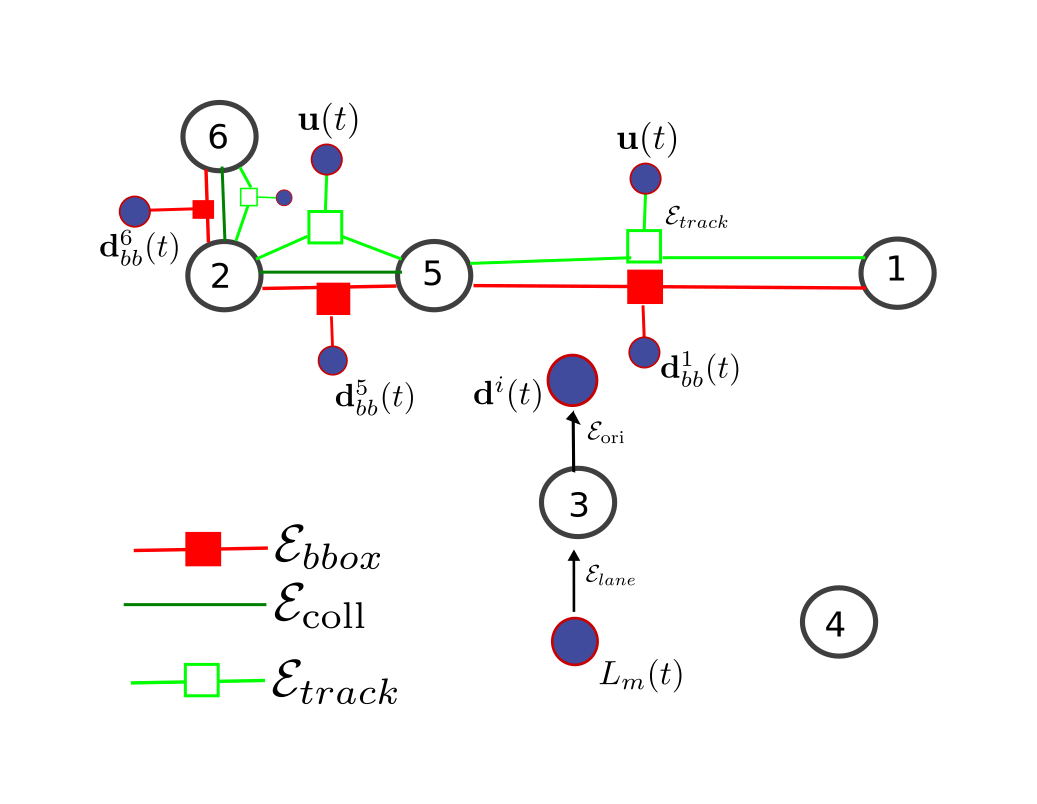
\includegraphics[width=\columnwidth]{Figures/graphicalModelFrom61ConstVars.pdf}
    %\tikzset{/tikz/x=0.8cm,/tikz/y=0.8cm}
  \begin{subfigure}[b]{0.55\textwidth}
    \usetikzlibrary{trees,shadows}
\providecommand{\Energy}[1]{E_{#1}}
\providecommand{\EnergyCol}{\Energy{col}}
\providecommand{\bb}[1]{d^{#1}(t)}
\providecommand{\trackp}[1]{u#1}
\providecommand{\pEnergy}[1]{E_{#1}}
\newcommand{\scenegraphicalmodel}{
  \begin{scope}[grow cyclic, line width=1.2,
      variablenode/.style={circle,circular drop shadow,draw=red,fill=white,thick},
      bboxfactor/.style= {rectangle,inner sep=2,fill=green!50!black,thick,text=green!50!black},
      collfactor/.style= {rectangle,inner sep=2,fill=blue,thick,text=blue},
      trackfactor/.style={rectangle,inner sep=2,fill=red,thick,text=red},
      obs/.style={fill=gray!30,draw=black,text=gray!30},
      prevf/.style={draw=green!20,text=gray},
      prevobsv/.style={draw=gray!10,fill=gray!1,text=gray},
      prevv/.style={draw=red!20,text=gray}
    ]
    \path[use as bounding box,clip] (-2.6, -4.5) rectangle (6.1,0.5);
    \draw (-2.5,-2.65) rectangle +(0.5,0.3);
    \draw (-2.0,-2.35) -- ++(0.15, 0.15) -- ++(0, -0.6) -- (-2.0, -2.65);
    \path
    (0, 0)  node [variablenode] (x6) {6}
    ++(0, -1.5) node [variablenode] (x2) {2}
    ++(2.5, 0)  node [variablenode] (x5) {5}
    +(.5, -2)   node [variablenode] (x3) {3}
    +(2.3, -2.5)   node [variablenode] (x4) {4}
    +(2.5, 0)  node [variablenode] (x1) {1}
    ;
    \path (x5)
    +(0, 1.5)  node [variablenode,obs] (u) {\tiny{1}}
    +(.2,0.9)  node {$\{\bu_j(t)\}$};

    % trackfactor
    \draw (x6) edge [bend left=40] node [trackfactor] (ft26) {\tiny{1}} (x2);
    \draw (ft26) edge [bend left=10] (u);
    \draw (x2) edge [bend left=35] node [trackfactor] (ft25) {\tiny{1}} (x5);
    \draw (ft25) edge (u);
    \draw (x5) edge [bend left=35] node [trackfactor] (ft51) {\tiny{1}} (x1);
    \draw (ft51) edge [bend right=35] (u);

    % bboxfactors
    \draw (x6) edge [bend right=40] node [bboxfactor] (f26) {\tiny{1}} (x2);
    \path (f26) +(-0.75,0) node [variablenode,obs] (d6) {\tiny{1}} 
    +(-.7,-.8)  node {$\textbf{d}^6(t)$};
    \draw (f26) edge (d6);
    \path (x2) ++(0,-1.25) node [variablenode,obs] (d2) {\tiny{1}} 
    +(-.8,0)  node {$\textbf{d}^2(t)$};
    \draw (x2) edge node [bboxfactor] {\tiny{1}} (d2);
    \draw (x2) edge [bend right=35] node [bboxfactor] (f25) {\tiny{1}} (x5);
    \path (x5) ++(-1.25,-1.25) node [variablenode,obs] (d5) {\tiny{1}} 
    +(.8,0)  node {$\textbf{d}^5(t)$};
    \draw (f25) edge (d5);
    \draw (x5) edge [bend right=35] node [bboxfactor] (f51) {\tiny{1}} (x1);
    \path (x1) ++(-1.25,-1.25) node [variablenode,obs] (d1) {\tiny{1}} 
    +(.8,0.2)  node {$\textbf{d}^1(t)$};
    \draw (f51) edge (d1);
    % \path (x3) ++(0,-1.25) node [variablenode,obs] (d3) {\tiny{1}} 
    % +(.8,0)  node {$\bb{3}$};
    % \draw (x3) edge node [bboxfactor] {\tiny{1}} (d3);
    % \path (x4) ++(0,1.25) node [variablenode,obs] (d4) {\tiny{1}} 
    % +(.8,0)  node {$\bb{4}$};
    % \draw (x4) edge node [bboxfactor] {\tiny{1}} (d4);

    % colfactor
    %% \draw (x6) edge node [collfactor] {\tiny{1}} (x2);
    %% \draw (x2) edge [] node [collfactor] {\tiny{1}} (x5);
    %% \draw (x5) edge [] node [collfactor] {\tiny{1}} (x1);

    % Legend
    \path (-1.75,-3.5) node (l1s) {} (-0, -3.5) node [anchor=west] (l1e) {$\Energy{detect}$};
    \draw (l1s) edge node [bboxfactor] {\tiny{1}} (l1e);
    % \path (-1.75,-4.5) node (l2s) {} (0, -4.5) node [anchor=west] (l2e) {$\EnergyCol$};
    %% \draw (l2s) edge node [collfactor] {\tiny{1}} (l2e);
    \path (-1.75,-4.2) node (l3s) {} (0, -4.2) node [anchor=west] (l3e) {$\EnergyTrack$};
    \draw (l3s) edge node [trackfactor] {\tiny{1}} (l3e);

  \end{scope}
}
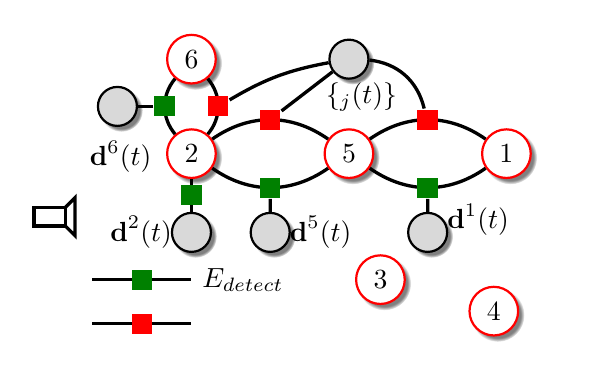
\begin{tikzpicture}
  \scenegraphicalmodel
\end{tikzpicture}

    \caption{Graphical model for a single frame with state of car represented
    as single node.}
  \end{subfigure}
  \begin{subfigure}[b]{0.45\textwidth}
    \tikzset{/tikz/x=0.8cm,/tikz/y=0.8cm}
    \usetikzlibrary{trees,shadows}
\providecommand{\Energy}[1]{E_{#1}}
\providecommand{\pEnergy}[1]{E_{#1}}
\providecommand{\EnergyCol}{\Energy{col}}
\providecommand{\relp}[2]{\mathbf{p}_{#1}({#2})}
\providecommand{\dimsn}[1]{\mathbf{B}^{#1}}
\providecommand{\bb}[1]{d^{#1}(t)}
\providecommand{\trackpit}[2]{\mathbf{u}^{(#1)}(#2)}
\begin{tikzpicture}[grow cyclic, line width=1.2,
    variablenode/.style={circle,circular drop shadow,draw=red,fill=white,thick,text=black},
    sizefactor/.style= {rectangle,inner sep=2,fill=magenta  ,thick,text=magenta},
    dynfactor/.style=  {rectangle,inner sep=2,fill=orange   ,thick,text=orange},
    lanefactor/.style= {rectangle,inner sep=2,fill=cyan    ,thick,text=cyan},
    trackfactor/.style={rectangle,inner sep=2,fill=red   ,thick,text=red},
    bboxfactor/.style= {rectangle,inner sep=2,fill=green!50!black,thick,text=green!50!black},
    level distance=30,
  obs/.style={fill=gray!30,text=gray!30,draw=black},
  prevf/.style={draw=green!20,text=gray},
  prevobsv/.style={draw=gray!10,fill=gray!1,text=gray},
  prevv/.style={draw=red!20,text=gray}
]
  \path[use as bounding box,clip] (-4.9, -4) rectangle (3.7,2.5);


  \path
  (-2.5,0) node[variablenode](dim) {2}
  +(-0.85, 0) node {$\dimsn{2}$};
  \visible<4->{
    \path (dim)
    +(-0.75,0.75) node[sizefactor](fsize){\tiny{2}}
    ;
    \draw (fsize) -- (dim);
  }

  \begin{scope}[line width=0.5]
    \path 
    % t-1 layer
    (1.5,1.5) node [variablenode] (xt1) {2}
    +(-0.20, 0.20) node[anchor=south east] {$\relp{2}{t-1}$}
  %  [counterclockwise from=-100,sibling angle=60]
  %  +(1.0, -1.0) node [factor,prevf] (flane1) {$E_{lane}$} 
  %  child { node [variablenode,obs,prevobsv] (l1) { $L_t$ } }
  %  child { node [ variablenode,obs,font=\footnotesize,prevobsv] (gps1) {GPS}}
  %  child { node [ variablenode,obs,font=\footnotesize,prevobsv] (map1) {Map}}

  %  [counterclockwise from=220]
  %  +(-1.0, -1.0) node[factor,prevf](fpt1) {$E_{pt}$}
  %  child { node[variablenode,obs,prevobsv](pt1){$u_t$} }

  %  [counterclockwise from=60,sibling angle=60]
  %  +(-1, 1.0) node[factor,prevf](fdet1){$E_{det}$} 
  %   child {
  %     node[variablenode,obs,prevobsv](gp1){$G_t$} 
  %   }
  %   child { node[variablenode,obs,prevobsv](Det1){$D_t$}
  %   }

    ;

  %\draw [gray](xt1) -- (fdet1) -- (dim);
  %\draw [gray](xt1) -- (flane1);
  %\draw [gray](xt1) -- (fpt1);
      
  \end{scope}

   %(0.5,1.0) node [dynfactor] (fdynx) {}
  %(1.95,1.8) node [factor,draw=gray,text=gray,minimum width=3] (fdynt) {$E_{d}$}

 %(0.2,2.0) node[factor](fhol) {$E_{hol}$}

  %(1, 0)  node[variablenode](theta){$\theta_t$}
  \draw
  (-1, 0)  node[variablenode](xt) {2}
  + (1.10, 0) node {$\relp{2}{t}$};
  \path 
  (-1.75, .75) node[bboxfactor](fdet){\tiny{2}} ;
  \path (-1.75, -.75) node[trackfactor] (fpt) {\tiny{2}};

  \draw (fpt) 
  ++(-90:1) node[variablenode,obs](pt){2} +(-.95,0) node {$\trackpit{2}{t}$} 
  ;
  \draw (xt) -- (fpt) -- (dim);
  \draw (fpt) -- (pt);
  \draw (fpt) edge [out=10,in=-110,gray] (xt1);
  \visible<3->{
    \draw (xt) edge node [dynfactor] (fdynx) {\tiny{2}} (xt1);
    \draw (xt) -- (fdynx) -- (xt1);
  }

  \visible<2->{
    \path (xt)
    ++ (0.75, -0.75) node [lanefactor] (flane) {\tiny{2}} ;
    %--
    %+ (-10:1) node [variablenode,obs] (l) {2} 
    % +(-10:1.8) node { $L_t$ } ;
    \draw (flane) --
    + (-45:1) node [ variablenode,obs,font=\footnotesize] (gps) {2} +(-60:1.7) node {$\{L_m\}$};
    %\draw (flane) -- +(-110:1)node [ variablenode,obs,font=\footnotesize] (map) {2} +(-110:1.7) node {Map};
    \draw (xt) -- (flane);
  }


 %++(65:1) node[variablenode,obs](gp){2} +(.75,0) node {$G_t$} ;
  \draw (fdet)
  --
  ++(90:1) node[variablenode,obs](Det){2} +(-.95,0) node {$\bb{2}$};
  \draw (xt) -- (fdet) -- (Det);
  
  %\path  (fpt) edge (theta);
  %\draw (fdet) -- (gp);
 %(0.2,2.0) node[factor](fhol) {$E_{hol}$}
  %\draw (xt) edge [bend left=40] node[factor] (fhol) {$E_{hol}$} (xt1);
  %\draw (fhol) -- (theta);  	  
  \draw (dim) -- (fdet);
  %\draw (theta) -- (flane);
  %\draw (theta) -- (fdynt) -- (theta1);
\coordinate (oneR) at (1.5,0);
\coordinate (oneRs) at (1,0);
  % Legend
  \visible<4->{
    \path (-3.8, -3.0) node (ls) {}
    ++(oneRs) node [anchor=west] (e1e) {$\EnergySize$};
    \draw (ls)  edge node [sizefactor] {\tiny{2}} (e1e) ;
  }
  \visible<3->{
    \path (e1e)
    ++(oneRs) node [] (e2s) {}
    ++(oneRs) node [anchor=west] (e2e) {$\EnergyDyn$};
    \draw (e2s) edge node [dynfactor] {\tiny{2}} (e2e) ;
  }
  \visible<2->{
    \path (e2e)
    ++(oneRs) node [] (e3s) {}
    ++(oneRs) node [anchor=west] (e3e) {$\EnergyLane$};
    \draw (e3s) edge node [lanefactor] {\tiny{2}} (e3e) ;
  }
\path (-3.8, -3.5)
  ++(oneRs) node [] (e4s) {}
  ++(oneRs) node [anchor=west] (e4e) {$\EnergyTrack$}
 ++(oneRs) node [] (e5s) {}
  ++(oneRs) node [anchor=west] (e5e) {$\EnergyBBox$}
  ;
  \draw (e4s) edge node [trackfactor] {\tiny{2}} (e4e) ;
  \draw (e5s) edge node [bboxfactor] {\tiny{2}} (e5e) ;
\end{tikzpicture}

    \caption{Factor graph dependence split up by pose and dimension}
  \end{subfigure}
\caption{Graphical model. The six numbered nodes represent the unknown state variables of each car. The shaded nodes in the graphical model are observed variables. %(1) Bounding box energy: The bounding box energy ($\Energy{bbox}$) without occlusion modeling is a unary term, but with occlusion it becomes a higher order term that affects the state of occluder as well. The bounding box detection is represented by $\mathbf{d}_{bb}^i(t)$. We can see that the bounding box energy affects both occluder and the occluded. (2) Point tracks energy ($\Energy{track}$) also exhibits occluder-occluded dependency.  The available point tracks are modeled by $\mathbf{u}(t)$. (3) Collision energy ($\Energy{coll}$) should ideally be globally dependent on all traffic participants but here we represent collision among only those TP that are near enough to have a significant collision energy. (4) Orientation from lane (and map) information ($\Energy{lane}$) depends only on single traffic participant hence show in the right subfigure. (5) Dynamic energies ($\Energy{dyn}$) also affect only one traffic participant at a time but over two frames. (6) Size prior ($\Energy{size}$) is used to enforce reasonable size of traffic participants.
}
  \label{fig:graphmodel}
\end{figure}
\begin{figure}
  \centering
\end{figure}


%%%%%%%%% BODY TEXT
\paragraph{The Model}

The objective is to find the most likely traffic participant (TP) state $\state{i}{t}$ given
various evidences $\mathbb{E} = \{\{\trackp{t}\}, \{\bb{i}\}, \{L_m\}\}$. This problem can be formulated as to find the states that maximize the conditional probability given the evidence,
%
\begin{align}
  \{\state{i}{t}\}^* &= \arg \max P(\{\state{i}{t}\} | \mathbb{E})\enspace.
\end{align}
%
By applying Bayes rule we get
\begin{align}
  P(\{\state{i}{t}\} | \mathbb{E}) &=
  \frac{1}{Z}P( \mathbb{E} | \{\state{i}{t}\})P(\{\state{i}{t}\}).
\end{align}
%
Assume conditional independence according to graphical model in Figure~\ref{fig:graphmodel}, we get an equivalant factorization of the joint probability distribution
%
\begin{multline}
  P(\{\state{i}{t}\} | \mathbb{E}) =
  \frac{1}{Z}
  \prod_{t=s_i}^{e_i}
  \left(
  \prod_{i,j: i \ne j}
  P(\state{i}{t}, \state{j}{t})
  P(\bb{i} | \state{i}{t}, \state{j}{t})
  P(\trackp{t} | \state{i}{t}, \state{j}{t})
\right)
\\
\left(
  \prod_{i=1}^{N}
  P(L_m(t) | \state{i}{t})
  P(\state{i}{t} | \state{i}{t-1})
  P(\state{i}{t})
\right)
  \enspace ,
\end{multline}
where $\bb{i}$ are the car detections, $\trackp{t}$ are the point tracks, $L_m(t)$ is the lane information from lane detection or GPS and Map information.
For computational reason it is common to work on factor graphs in log domain
and for historical reasons the negative log of probability is also called the energy of the system. In energy domain our factorization simplifies to
%
\begin{multline}
  -\log{P(\{\state{i}{t}\} | \mathbb{E})} = 
  -Z' 
  + \sum_{t=s_i}^{e_i}
  \left(
  \sum_{i,j:i\ne j}   
  \WEnergyCol 
   + \WpEnergy{bbox}
   + \WpEnergy{track}
\right)
  \\
  + \left(
  \sum_{i=1}^N 
  \WEnergy{lane}
  + \WEnergy{dyn}
  + \WEnergy{size}
\right)
  \enspace.
\end{multline}
%
Here $\WEnergyCol = -\log P(\state{i}{t}, \state{j}{t})$ is collision energy which penalizes localization of cars that are too close together, $\WpEnergy{bbox} = -\log P(\bb{i} | \state{i}{t}, \state{j}{t})$ is bounding box energy that encourages the alignment of projected bounding box with the detected bounding box, $\WpEnergy{track} = -\log P(\trackp{t} | \state{i}{t}, \state{j}{t})$ is the point tracks energy which encourages the alignment of re-projected point tracks with ones that are detected, $\WEnergy{lane} = - \log P(L_m(t) | \state{i}{t})$ is lane energy which encourages cars to be along the direction of lanes, $\WEnergy{dyn} = - \log P( \state{i}{t} | \state{i}{t-1} ) $ is dynamic energy which captures the motion model of the cars and finally $\WEnergy{size} = - \log P (\state{i}{t})$ is the size prior over the cars. $\lambda_{\text{\{col,bbox,track,lane,dyn,size\}}}$ are unknown parameters that weight different energies. For now we set them empirically, but eventually they need to be learned from the data.
